% !TEX root = ../main.tex
\section{Ejercicio propuesto 2: pruebas diferenciales y análisis experimental}

\subsection{Entorno de pruebas y configuración}
Las pruebas experimentales se ejecutaron en un procesador AMD64 (8 núcleos / 16 hilos), 23.36 GB RAM, Windows 11 Pro 64 bits con Python 3.12.8 estándar (CPython). Fijamos la constante $\texttt{SEMILLA\_GLOBAL} = 2026$ para reproducir idénticamente los grafos, secuencias de enlace y mediciones con \texttt{time.perf\_counter}.

% -------------------------------------------------------------------------
\subsection{Escenario A: pruebas deterministas de la guía}
Evaluamos el árbol de 7 nodos de la guía con valores $v \in \{1..7\}$ y $\text{value}(v) \in \{4, 7, 2, 9, 1, 6, 3\}$, con las aristas $\{(1, 2), (1, 3), (2, 4), (2, 5), (3, 6), (3, 7)\}$ frente al oráculo BFS:

\begin{table}[H]
    \caption{Resultados del Escenario A frente al modelo de referencia BFS}
    \label{tab:escenario_a}
    \centering
    \footnotesize
    \begin{tabular*}{\textwidth}{@{\extracolsep{\fill}}lccc}
        \toprule
        \textbf{Operación evaluada} & \textbf{Esperado} & \textbf{Link-Cut Tree} & \textbf{Estado} \\
        \midrule
        \texttt{path\_sum(4, 5)}       & 17 & 17 & Correcto \\
        \texttt{path\_sum(4, 6)}       & 28 & 28 & Correcto \\
        \texttt{path\_sum(6, 7)}       & 11 & 11 & Correcto \\
        \texttt{cut(1, 3); connected(4, 6)} & False & False & Correcto (separado) \\
        \texttt{link(1, 3); path\_sum(4, 6)}& 28 & 28 & Correcto (reconectado) \\
        \texttt{path\_sum} con signos ($5 + 0 - 3$) & 2 & 2 & Correcto (soporta negativos) \\
        Rechazo de ciclo (\texttt{link(4, 6)}) & ValueError & ValueError & Interceptado \\
        Rechazo de corte falso (\texttt{cut(4, 6)}) & ValueError & ValueError & Interceptado \\
        \bottomrule
    \end{tabular*}
\end{table}

% -------------------------------------------------------------------------
\subsection{Escenario B: pruebas aleatorias diferenciales (15\,000 operaciones)}
Sometimos la estructura a $15\,000$ operaciones aleatorias ($5\,000$ por tamaño en $n \in \{30, 60, 120\}$) combinando \texttt{link}, \texttt{cut}, \texttt{connected}, \texttt{path\_sum} y \texttt{make\_root}, contrastando cada resultado contra el oráculo BFS:

\begin{table}[H]
    \caption{Conteo de operaciones diferenciales verificadas (Escenario B)}
    \label{tab:escenario_b}
    \centering
    \footnotesize
    \begin{tabular*}{\textwidth}{@{\extracolsep{\fill}}ccccccccc}
        \toprule
        $\mathbf{n}$ & \textbf{Total Ops} & \texttt{link} & \texttt{cut} & \texttt{connected} & \texttt{path\_sum} & \texttt{make\_root} & \textbf{Discrepancias} & \textbf{Invariantes} \\
        \midrule
        30  & 5\,000 & 1\,076 & 1\,048 & 1\,219 & 1\,233 & 424 & \textbf{0} & 5\,001 OK \\
        60  & 5\,000 & 1\,098 & 1\,041 & 1\,196 & 1\,251 & 414 & \textbf{0} & 5\,001 OK \\
        120 & 5\,000 & 1\,146 & 1\,039 & 1\,157 & 1\,248 & 410 & \textbf{0} & 5\,001 OK \\
        \midrule
        \textbf{Total} & \textbf{15\,000} & \textbf{3\,320} & \textbf{3\,128} & \textbf{3\,572} & \textbf{3\,732} & \textbf{1\,248} & \textbf{0} & \textbf{15\,003 OK} \\
        \bottomrule
    \end{tabular*}
\end{table}

\clearpage
% -------------------------------------------------------------------------
\begin{figure}[H]
    \centering
    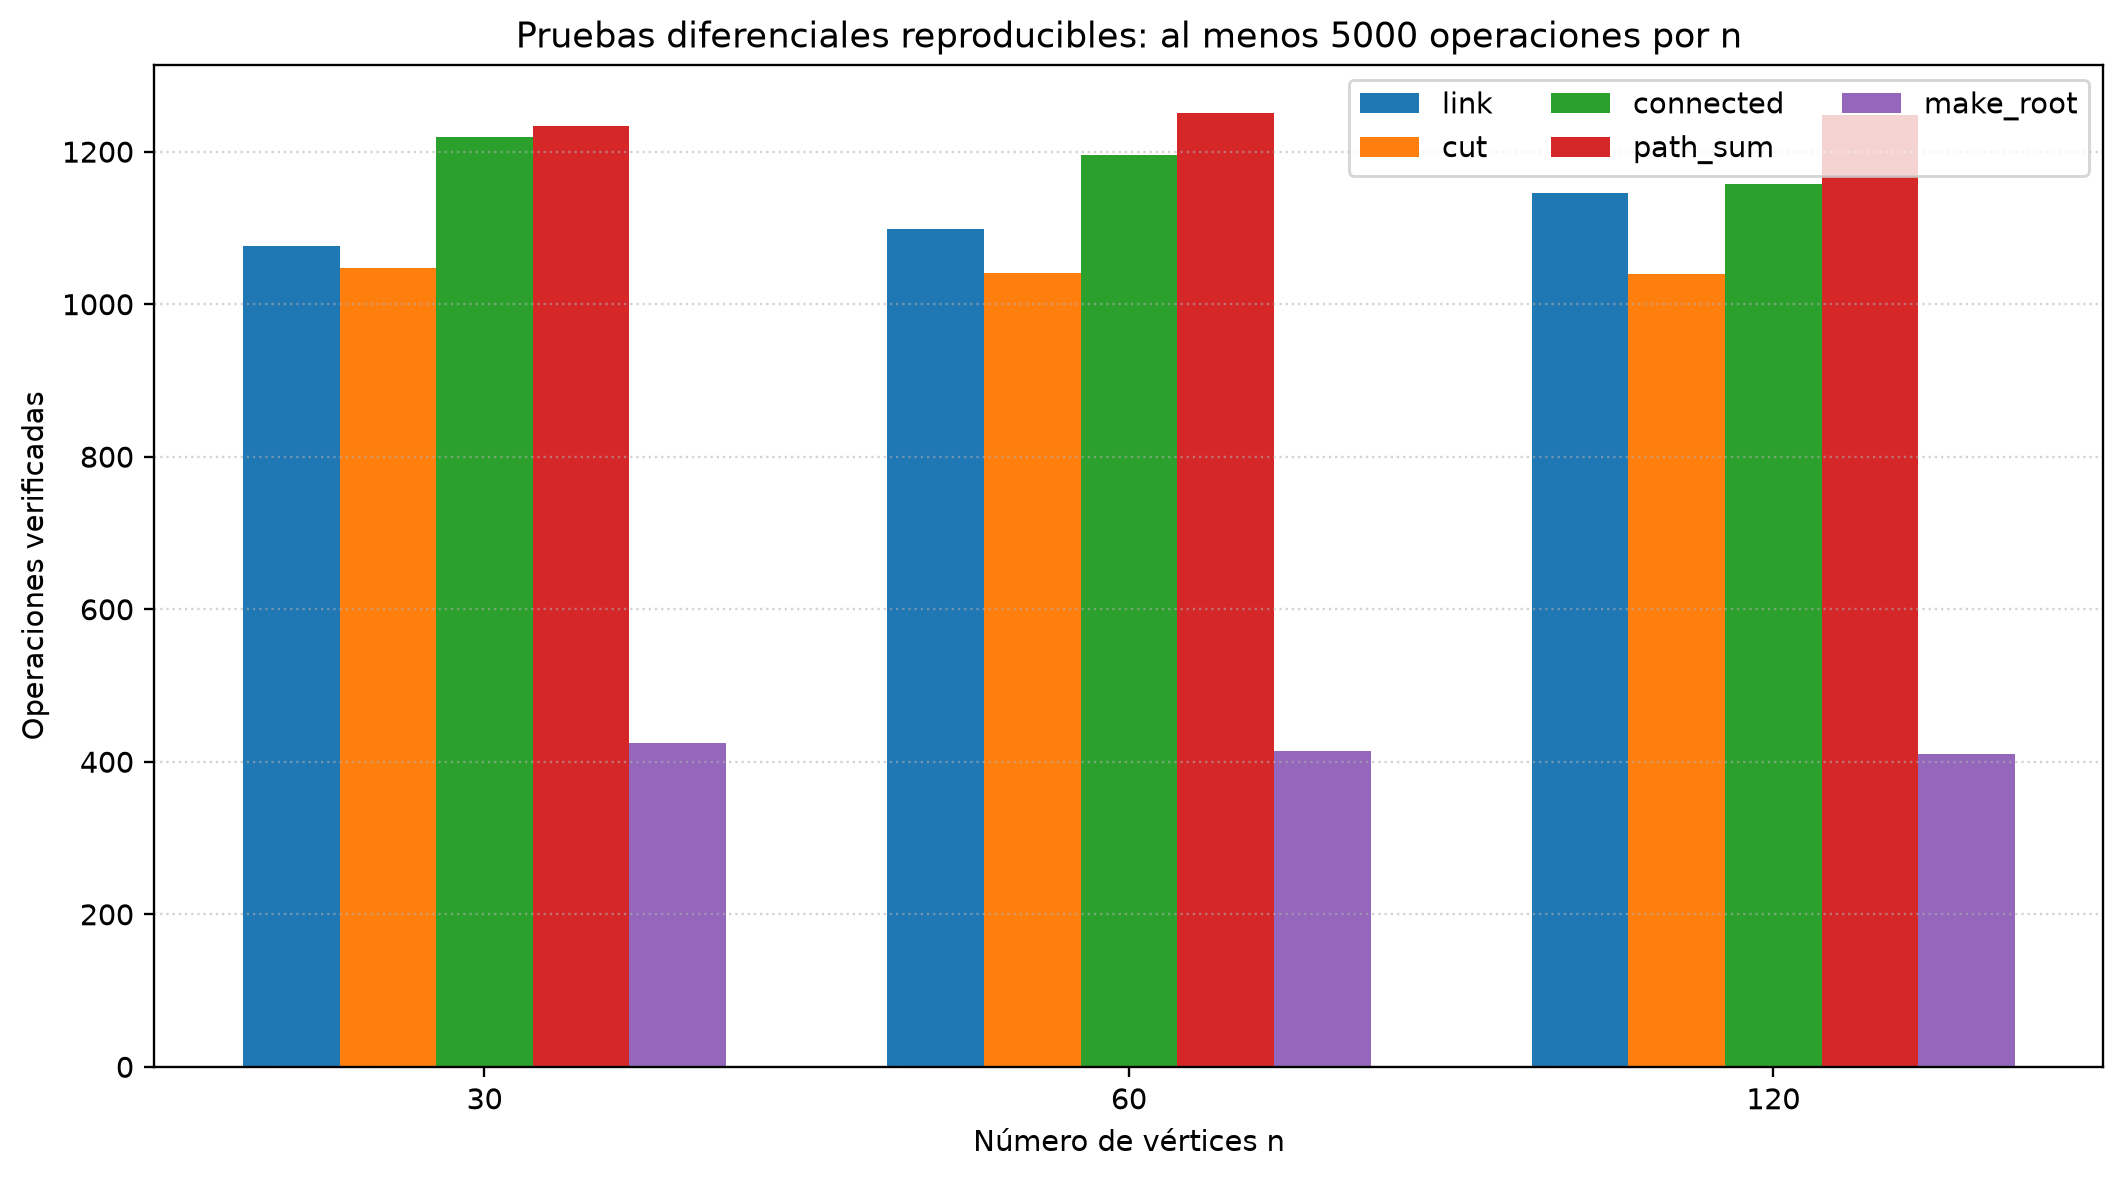
\includegraphics[width=\textwidth, keepaspectratio]{fig_pruebas_diferenciales.png}
    \caption{Operaciones diferenciales ejecutadas con 0 discrepancias frente a BFS}
    \label{fig:pruebas_diferenciales}
\end{figure}

El resultado arrojó \textbf{cero discrepancias en las 15\,000 operaciones}, y las 15\,003 validaciones de invariantes se mantuvieron en estado OK.

\subsection{Escenario C: pruebas de rendimiento por topología}
Evaluamos tres topologías para $n \in \{100, 200, 400, 800, 1\,600\}$: (1)~\textbf{Cadena lineal:} caminos largos $O(n)$; (2)~\textbf{Estrella:} nodo central conectado a $n-1$ hojas (profundidad $\le 2$); y (3)~\textbf{Árbol aleatorio:} ramificación intermedia.

\begin{table}[H]
    \caption{Resumen de mediciones de rendimiento por topología (Escenario C)}
    \label{tab:escenario_c}
    \centering
    \scriptsize
    \setlength{\tabcolsep}{4pt}
    \begin{tabular*}{\textwidth}{@{\extracolsep{\fill}}llrrrrrr}
        \toprule
        $\mathbf{n}$ & \textbf{Topología} & \textbf{Tiempo (ms)} & \textbf{Rotaciones} & \textbf{Rot/Op} & \textbf{Splays} & \textbf{Exposes} & \textbf{Inversiones} \\
        \midrule
        100   & Cadena    & 46.19 & 5\,746  & 12.36 & 4\,565 & 1\,260 & 2\,542 \\
        100   & Estrella  & 33.30 & 3\,503  & 7.53  & 4\,392 & 1\,260 & 823    \\
        100   & Aleatorio & 54.09 & 5\,729  & 12.32 & 4\,943 & 1\,260 & 1\,645 \\
        \midrule
        400   & Cadena    & 70.99 & 7\,710  & 16.58 & 4\,976 & 1\,260 & 3\,373 \\
        400   & Estrella  & 36.58 & 3\,467  & 7.46  & 4\,385 & 1\,260 & 805    \\
        400   & Aleatorio & 52.63 & 6\,608  & 14.21 & 5\,249 & 1\,260 & 1\,810 \\
        \midrule
        1\,600 & Cadena    & 123.34 & 11\,151 & 23.98 & 6\,254 & 1\,260 & 4\,482 \\
        1\,600 & Estrella  & 67.48  & 3\,443  & 7.40  & 4\,383 & 1\,260 & 787    \\
        1\,600 & Aleatorio & 85.54  & 7\,615  & 16.38 & 5\,567 & 1\,260 & 1\,915 \\
        \bottomrule
    \end{tabular*}
\end{table}

\clearpage
% -------------------------------------------------------------------------
\subsection{Discusión de resultados experimentales}
\begin{itemize}\setlength\itemsep{0pt}\setlength\parskip{0pt}
    \item \textbf{¿Por qué la cadena tiene más rotaciones?} En la cadena lineal los caminos tienen longitud $O(n)$, obligando a enlazar múltiples auxiliares profundos ($23.98$ rot/op para $n=1\,600$). En la estrella, con profundidad 2, las rotaciones se mantienen constantes (${\approx} 7.4$ rot/op).
    \item \textbf{¿El tiempo en Python demuestra $O(\log n)$?} No directamente en tiempo de reloj por la sobrecarga del intérprete. La cota $O(\log n)$ se comprueba matemáticamente por el crecimiento logarítmico de las rotaciones y la función potencial de Sleator-Tarjan.
\end{itemize}

\begin{figure}[H]
    \centering
    \begin{subfigure}[b]{0.485\textwidth}
        \centering
        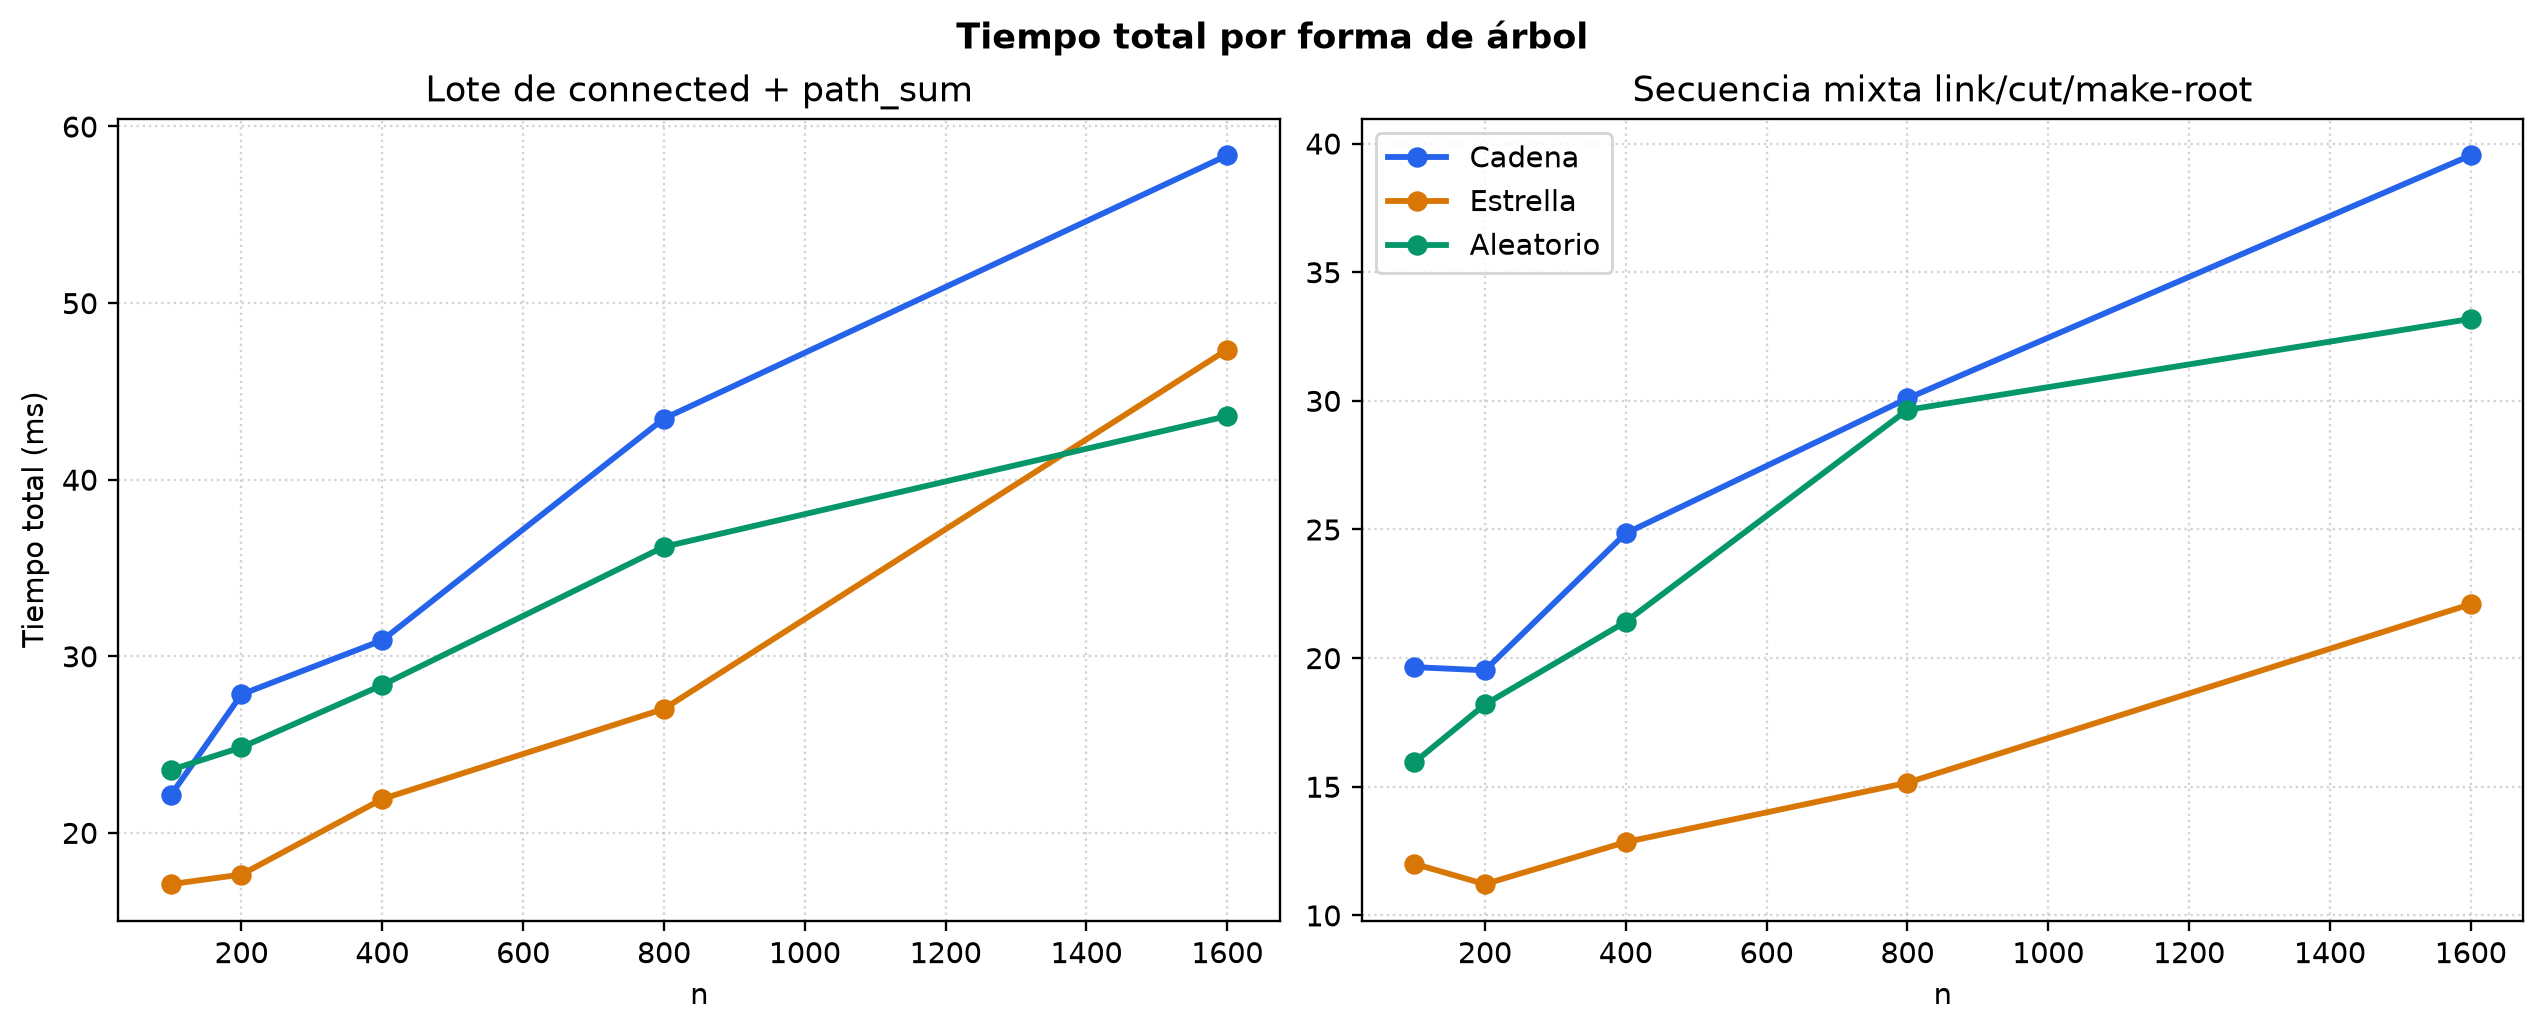
\includegraphics[width=\textwidth, keepaspectratio]{fig_tiempo_por_forma.png}
        \caption{Tiempo de ejecución frente a $n$}
    \end{subfigure}
    \hfill
    \begin{subfigure}[b]{0.485\textwidth}
        \centering
        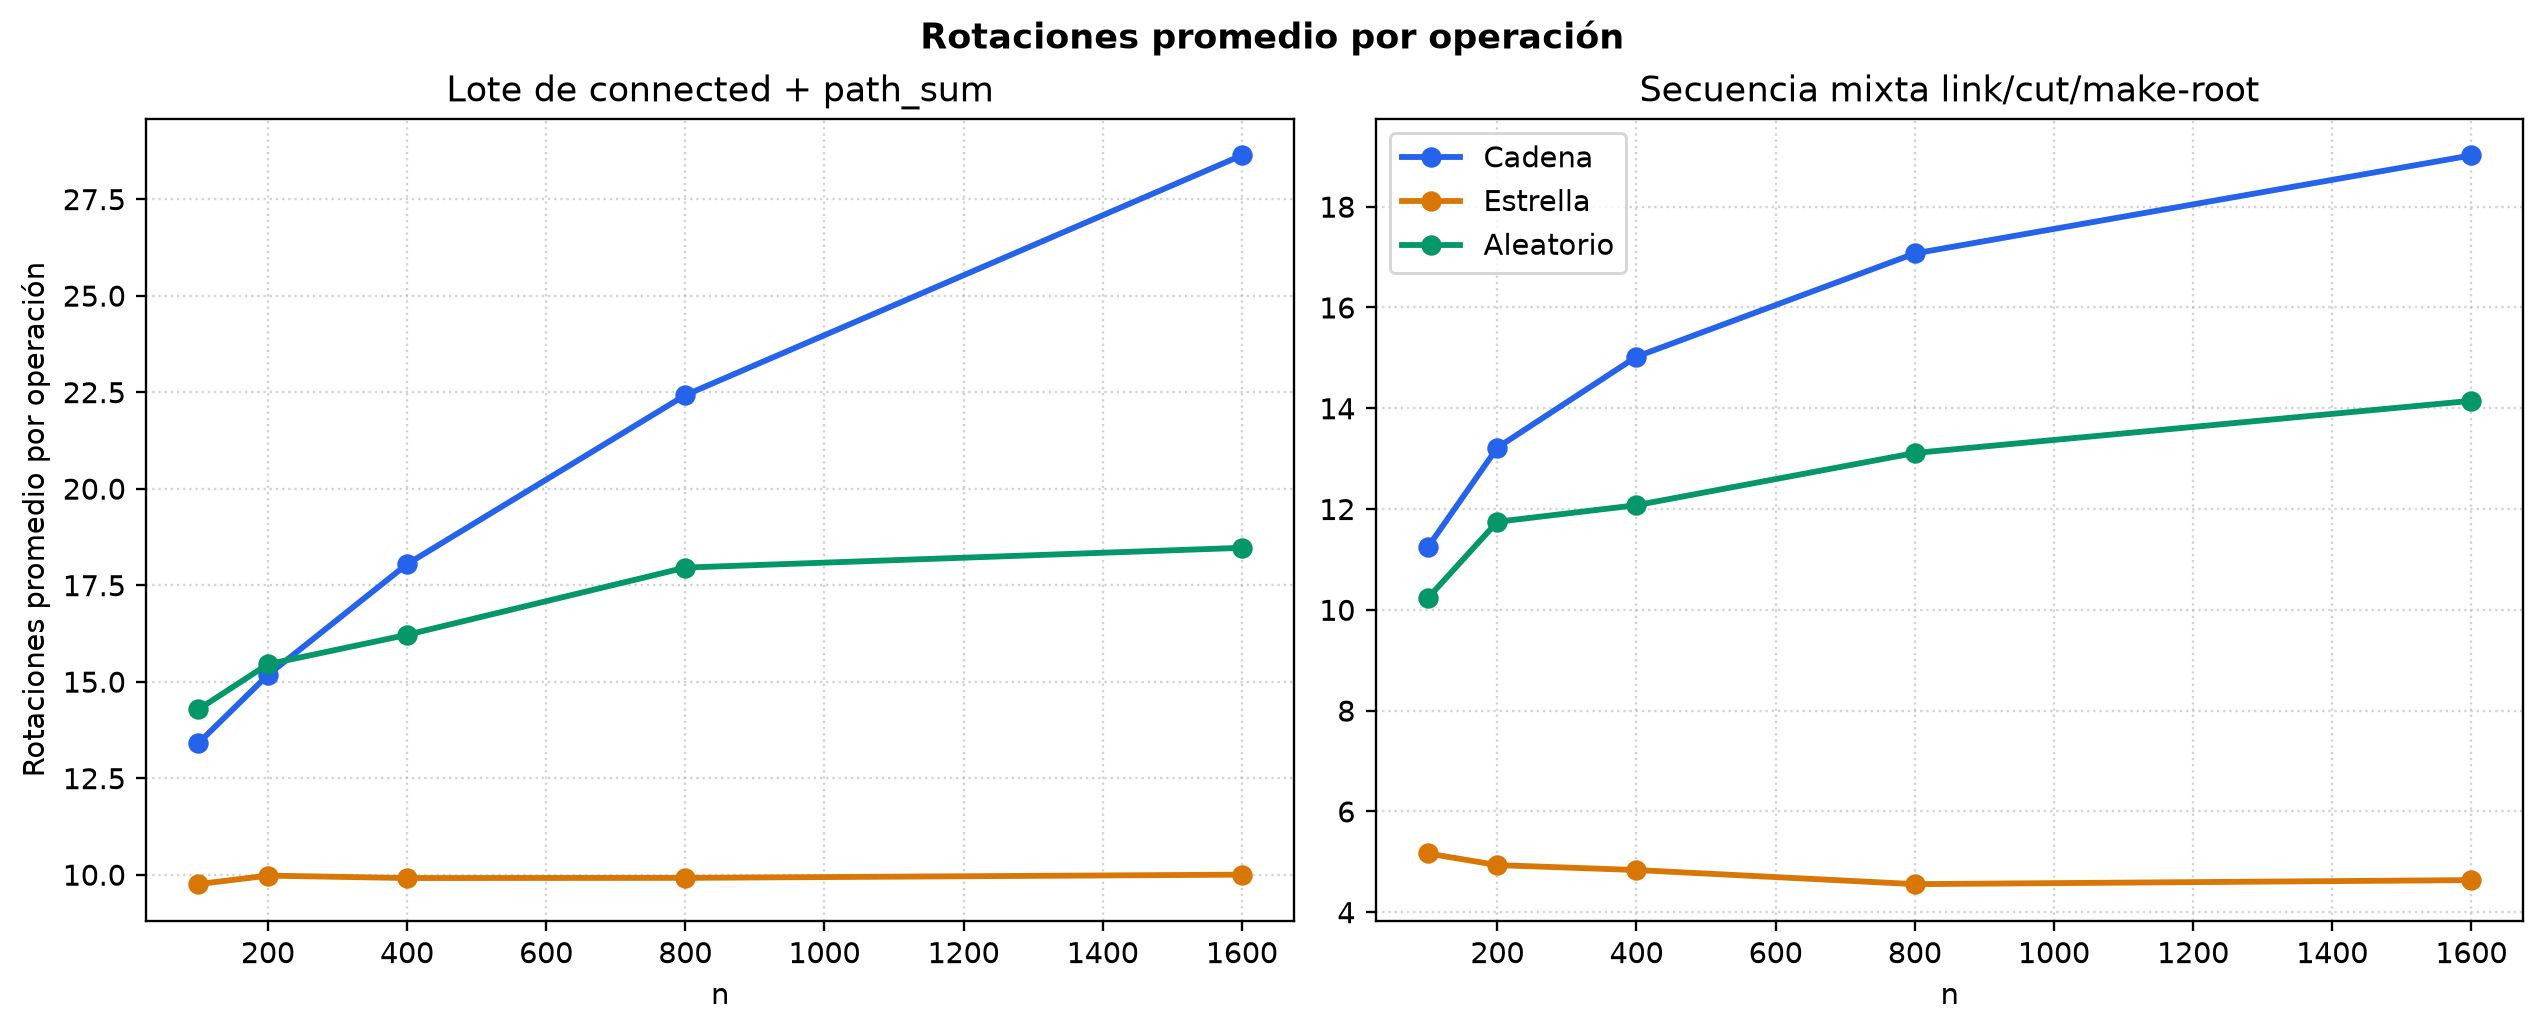
\includegraphics[width=\textwidth, keepaspectratio]{fig_rotaciones_promedio.png}
        \caption{Rotaciones promedio por operación}
    \end{subfigure}
    \caption{Rendimiento y rotaciones según la forma del árbol}
    \label{fig:experimentos_c}
\end{figure}

\begin{figure}[H]
    \centering
    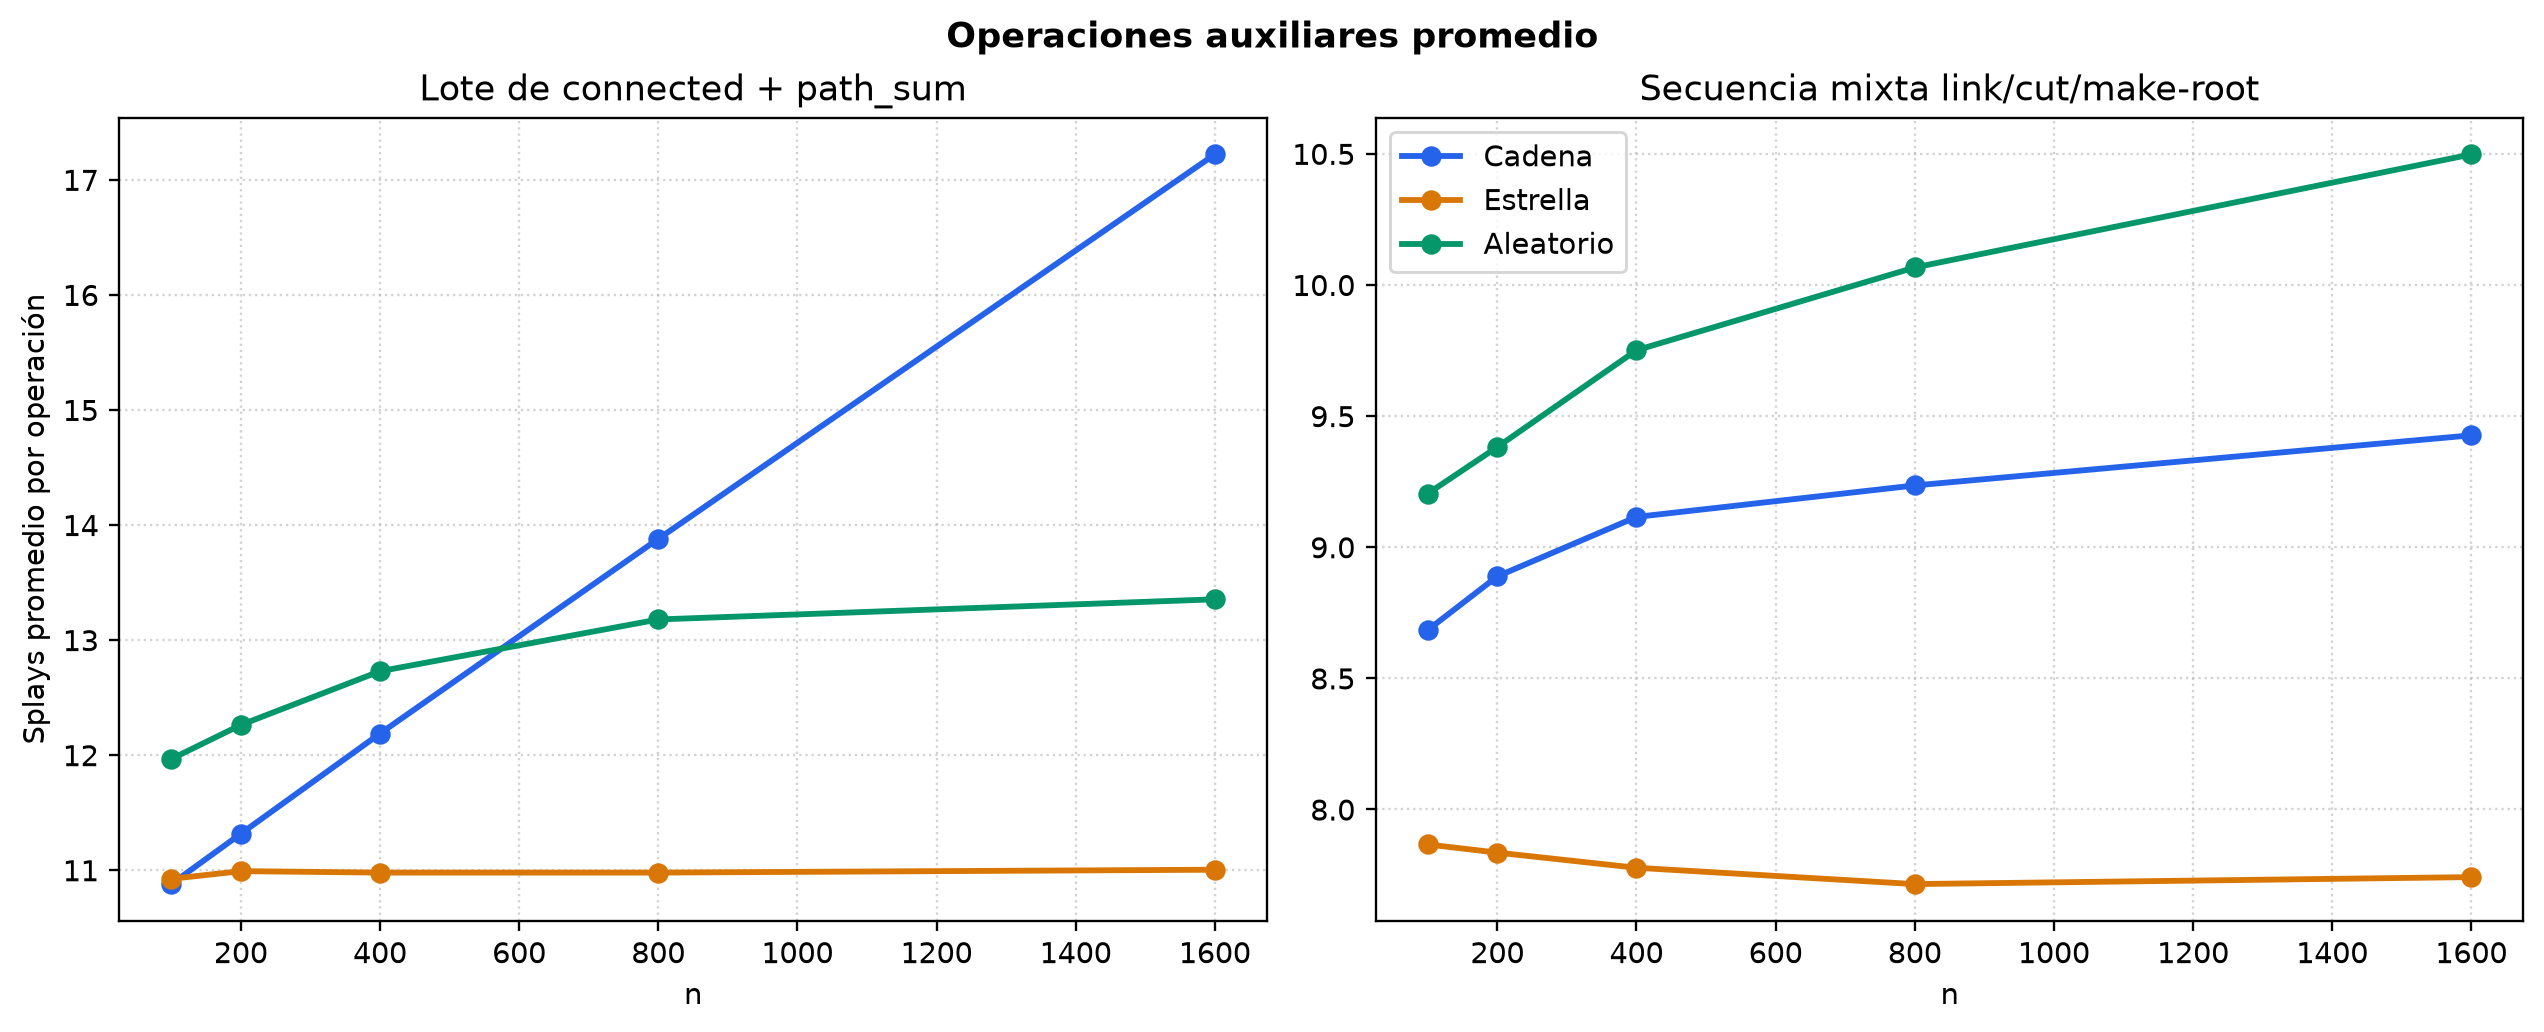
\includegraphics[width=0.92\textwidth, keepaspectratio]{fig_operaciones_auxiliares.png}
    \caption{Cantidad de splays, exposiciones e inversiones diferidas por tamaño}
    \label{fig:ops_auxiliares}
\end{figure}
